\documentclass[11pt]{beamer}
\usepackage[fontset=mac]{ctex}
\usepackage{hyperref}
\usepackage[T1]{fontenc}

\usepackage{latexsym,amsmath,xcolor,multicol,booktabs,calligra}
\usepackage{graphicx}
\usepackage{tikz}
\usepackage[RPvoltages]{circuitikz}
\usetikzlibrary{positioning,arrows.meta,fit,backgrounds}

\author{Yuanqi}
\title{基于接收波形的 Chiplet 晶粒间互连故障诊断}
\subtitle{多模态遥测的价值取决于观测的有损性}
\institute{清华大学 \quad VLSI 测试课程 Mini Research Project}
\date{2026 年 6 月 11 日}
\usepackage{Tsinghua}

\definecolor{deepred}{rgb}{0.6,0,0}
\definecolor{thublue}{RGB}{31,119,180}
\newcommand{\hl}[1]{\textcolor{deepred}{\textbf{#1}}}

\begin{document}

\kaishu

% ============================================================ title
\begin{frame}
    \titlepage
    \begin{tikzpicture}[remember picture,overlay]
        \node[anchor=south] at ([yshift=42pt]current page.south)
            {
\includegraphics[width=0.10\linewidth]{pic/Tsinghua_University_Logo.png}};
    \end{tikzpicture}
\end{frame}

\begin{frame}
    \tableofcontents[sectionstyle=show,subsectionstyle=hide]
\end{frame}

% ============================================================
\section{背景与问题}

\begin{frame}{为什么关注 D2D 互连的在役健康}
    \begin{columns}
        \column{0.31\textwidth}
            \centering
            {\Large\textbf{$\sim10^5$}}\\[-2pt]
            {\small 单封装 D2D 互连数}
        \column{0.31\textwidth}
            \centering
            {\Large\textbf{$<10\,\mu$m}}\\[-2pt]
            {\small 微凸点节距}
        \column{0.31\textwidth}
            \centering
            {\Large\textbf{部署后}}\\[-2pt]
            {\small 老化/漂移/翘曲失效}
    \end{columns}
    \vspace{0.8em}
    \begin{center}
        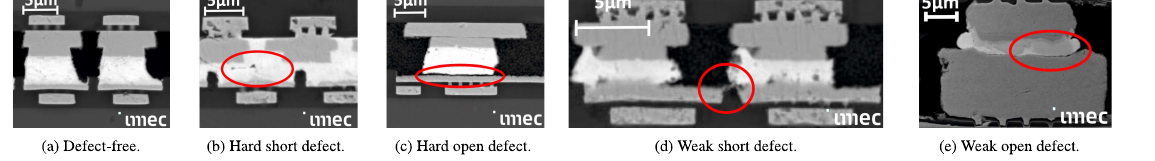
\includegraphics[width=0.98\textwidth]{pic/sem_bump_defects.png}\\[2pt]
        {\scriptsize 微凸点缺陷的 SEM 截面（imec，Wang et al., ETS 2024）：硬开路/短路之外还有\hl{弱（参数化）缺陷}}
    \end{center}
    \begin{itemize}
        \item 制造期结构测试（IEEE 1838 + 确定图案）是\hl{一次性}的 pass/fail
        \item 弱缺陷、老化与漂移表现为\hl{裕度的缓慢侵蚀}——只有在役监测能看到
    \end{itemize}
\end{frame}

\begin{frame}{相关工作：五条路线及其留下的空白}
    \centering
    \footnotesize
    \begin{tabular}{@{}p{2.1cm}p{4.6cm}p{3.6cm}@{}}
        \toprule
        \textbf{路线} & \textbf{代表做法} & \textbf{未覆盖之处} \\
        \midrule
        结构测试 BIST & IEEE 1838 + 条纹图案，常数级向量 & 制造期一次性，难覆盖在役退化 \\
        ML 互连诊断 & S 参数/眼图/TDR + CNN/SVM/AE & 固定图案、假设完整波形 \\
        老化监测 & 环振/路径监视器 + 寿命预测 & 芯片级指标，定位不到互连 \\
        热建模 & 电--热协同仿真 & 温度被当作待补偿外因 \\
        安全监测 & 延迟 PUF / 阻抗谱 & 不关注渐进退化 \\
        \bottomrule
    \end{tabular}
    \vspace{0.7em}
    \begin{block}{\small 四个空白（本文逐一用实验回应）}
        \small ① 环境量与故障征象的\hl{混杂}关系 \quad ② 运行时\hl{观测受限}\\
        ③ \hl{随机工作负载}下的泛化 \quad ④ 未知故障的\hl{开集}识别
    \end{block}
    \vspace{2pt}
    {\tiny 文献：Huang ITC'24；Chuang TCAD'25；Wang ETS'24；Cui ETS'23；Huang TCPMT'18；Kang arXiv'23；Medico EPEPS'18；Usama TCAD'26；Lanzieri arXiv'24；Ali IOLTS'20；Ortega ITC'25；Zhu arXiv'25；Ma TVLSI'24；Deric TCHES'22；Monfared arXiv'25}
\end{frame}

\begin{frame}{问题定义：同一条链路，两种观测体制}
    \centering
    \begin{tikzpicture}[
        box/.style={draw,rounded corners=2pt,align=center,font=\small,
                    minimum height=0.9cm,inner sep=5pt},
        arr/.style={-{Latex[length=2.5mm]},thick}]
        \node[box,fill=gray!15] (sim) {D2D 链路\\（随机工作负载）};
        \node[box,fill=thublue!15,right=0.9cm of sim] (wave) {接收端波形\\160 UI $\times$ 8 采样};
        \node[box,fill=green!12,above right=0.05cm and 1.1cm of wave] (full)
            {\textbf{完整波形}（bring-up / 后硅）\\1280 点全部可见};
        \node[box,fill=red!12,below right=0.05cm and 1.1cm of wave] (lossy)
            {\textbf{有损标量}（运行时）\\单个眼裕度数字};
        \node[box,fill=yellow!20,below=0.45cm of wave] (tel) {片上遥测：温度、droop\\（DTS / droop monitor，已常态化）};
        \draw[arr] (sim) -- (wave);
        \draw[arr] (wave.east) -- (full.west);
        \draw[arr] (wave.east) -- (lossy.west);
        \draw[arr,dashed] (tel.east) -| ($(lossy.south west)+(0.4,0)$);
    \end{tikzpicture}
    \vspace{0.6em}
    \begin{itemize}
        \item 任务：10 类故障诊断（含并发）、连续严重度回归、健康/故障报警
        \item 难点：温度与供电 droop \hl{同样闭合眼图}——良性扰动与缺陷征象重叠
        \item \hl{核心问题}：加入温度/droop 遥测，到底什么时候有用？
    \end{itemize}
\end{frame}

% ============================================================
\section{仿真平台与数据集}

\begin{frame}{纯 ngspice 的 D2D 链路仿真器（完全可复现）}
    \centering
    \resizebox{0.93\textwidth}{!}{%
    \begin{circuitikz}[american,line width=0.7pt,every label/.style={font=\scriptsize}]
    \def\gnd{-2.0}
    \draw (0,0) to[V=$v_\text{drv}$] (0,\gnd) node[ground]{};
    \draw (0,0) to[R=$R_\text{on}(T)$] (2.4,0) coordinate(txo);
    \draw[dashed,gray] (2.55,-0.6) rectangle (5.05,0.6);
    \node[gray] at (3.75,0.95) {\scriptsize TX 微凸点};
    \draw (txo) to[R=$R_b$] (3.75,0) to[L=$L_b$] (5.0,0) coordinate(n0);
    \draw (n0) to[C=$C_b$] (5.0,\gnd) node[ground]{};
    \draw (n0) to[R=$R_\text{seg}$] (6.7,0) coordinate(nm) to[L=$L_\text{seg}$] (8.3,0) coordinate(nk);
    \draw (8.3,0) to[C=$C_\text{node}$] (8.3,\gnd) node[ground]{};
    \draw (nm) to[C=$C_c$] (6.7,1.7) node[above]{\scriptsize aggressor};
    \draw[gray,|-|] (5.0,-2.55) -- (8.3,-2.55);
    \node[gray,below=0pt] at (6.65,-2.6) {\scriptsize $N{=}20$ 段 RLGC 阶梯};
    \draw (nk) -- (8.65,0);  \draw (9.35,0) -- (9.7,0) coordinate(nN);
    \node at (9.0,0) {\large$\cdots$};
    \draw[dashed,gray] (9.75,-0.6) rectangle (12.25,0.6);
    \node[gray] at (10.95,0.95) {\scriptsize RX 微凸点};
    \draw (nN) to[R=$R_b$] (10.95,0) to[L=$L_b$] (12.2,0) coordinate(rxo);
    \draw (rxo) to[C=$C_\text{rx}$] (12.2,\gnd) node[ground]{};
    \draw (rxo) -- (14.4,0) coordinate(rt);
    \node[above] at (13.3,0.15) {\scriptsize 采样 $v$(rxo)};
    \draw (rt) to[R=$R_\text{term}$] (14.4,\gnd);
    \draw (14.1,\gnd) -- (14.7,\gnd);
    \node[below=1pt] at (14.4,\gnd) {\scriptsize $V_\text{dd}/2$};
    \end{circuitikz}}
    \vspace{0.4em}
    \begin{itemize}\small
        \item UCIe 级参数：16 GT/s、0.8 V 低摆幅单端、2 mm、两条邻线串扰
        \item 四项物理扩展：\hl{热噪声}$\propto\sqrt{TR}$、\hl{$R_\text{on}(T)$}（温度闭眼主机制）、\hl{连续漂移故障 + 良性 droop}、\hl{TX 抖动}（RJ/DCD/SJ）
    \end{itemize}
\end{frame}

\begin{frame}{十类故障：每类是一个带严重度轴的电路参数偏移}
    \begin{figure}
        \centering
        
\includegraphics[height=0.8\textheight]{pic/eyes.png}
    \end{figure}
\end{frame}

\begin{frame}{数据集 v2：采样一个操作空间，而非枚举网格}
    \begin{figure}
        \centering
        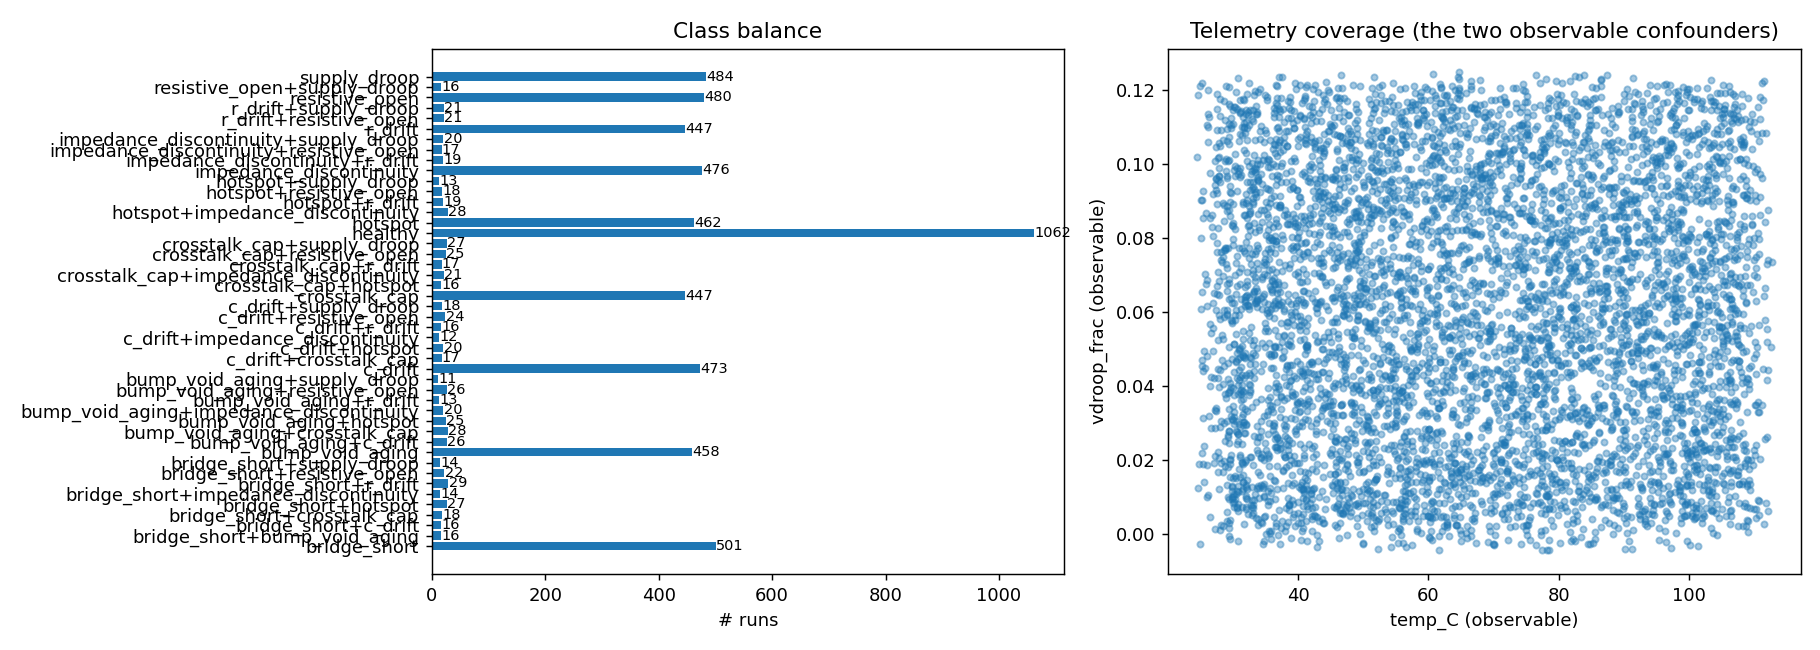
\includegraphics[width=0.92\textwidth]{pic/overview_v2.png}
    \end{figure}
    \begin{itemize}\small
        \item 6000 条；温度 $T\sim U(27,110)^\circ$C \hl{对所有类同分布}（杜绝标签捷径）
        \item 码型逐样本随机（PRBS 种子）；信道制造偏差、TX 抖动作为滋扰
        \item 15\% 样本双故障并发；8 进程并行 ngspice，全集 20 分钟生成
    \end{itemize}
\end{frame}

% ============================================================
\section{方法与结果}

\begin{frame}{诊断通路：从波形到判决}
    \centering
    \resizebox{0.98\textwidth}{!}{%
    \begin{tikzpicture}[
        box/.style={draw,rounded corners=2pt,align=center,font=\small,
                    minimum height=0.85cm,inner sep=4pt},
        arr/.style={-{Latex[length=2.5mm]},thick}]
        \node[box,fill=gray!15] (in) {RX 波形\\$1\times1216$};
        \node[box,fill=thublue!15,right=0.55cm of in] (c1) {Conv 16};
        \node[box,fill=thublue!25,right=0.45cm of c1] (c2) {Conv 32};
        \node[box,fill=thublue!35,right=0.45cm of c2] (c3) {Conv 64};
        \node[box,fill=thublue!15,right=0.45cm of c3] (pool) {mean+max\\池化};
        \node[box,fill=green!15,right=0.55cm of pool] (fc) {全连接};
        \node[box,fill=yellow!20,below=0.5cm of pool] (tel) {遥测 [T, droop]（可选）};
        \node[box,fill=red!12,above right=0.45cm and 0.7cm of fc] (h1) {\scriptsize 10 类 softmax};
        \node[box,fill=red!12,right=0.7cm of fc] (h2) {\scriptsize 9 位多标签};
        \node[box,fill=red!12,below right=0.45cm and 0.7cm of fc] (h3) {\scriptsize 严重度回归};
        \draw[arr] (in) -- (c1); \draw[arr] (c1) -- (c2); \draw[arr] (c2) -- (c3);
        \draw[arr] (c3) -- (pool); \draw[arr] (pool) -- (fc);
        \draw[arr,dashed] (tel) -| (fc);
        \draw[arr] (fc) -- (h1.west); \draw[arr] (fc) -- (h2); \draw[arr] (fc) -- (h3.west);
    \end{tikzpicture}}
    \vspace{0.6em}
    \begin{itemize}\small
        \item $z$ 标准化、丢弃前 8 个填充比特；区域掩膜由\hl{每行自己的发送比特}重建
        \item 多标签头在验证集上做\hl{逐类阈值校准}（报警阈值校准 = 生产监控常规）
        \item 对照基线：眼裕度标量规则、18 维人工特征、原始波形逻辑回归、LSTM
    \end{itemize}
\end{frame}

\begin{frame}{主结果：哪一级观测 + 哪种模型才够用}
    \begin{figure}
        \centering
        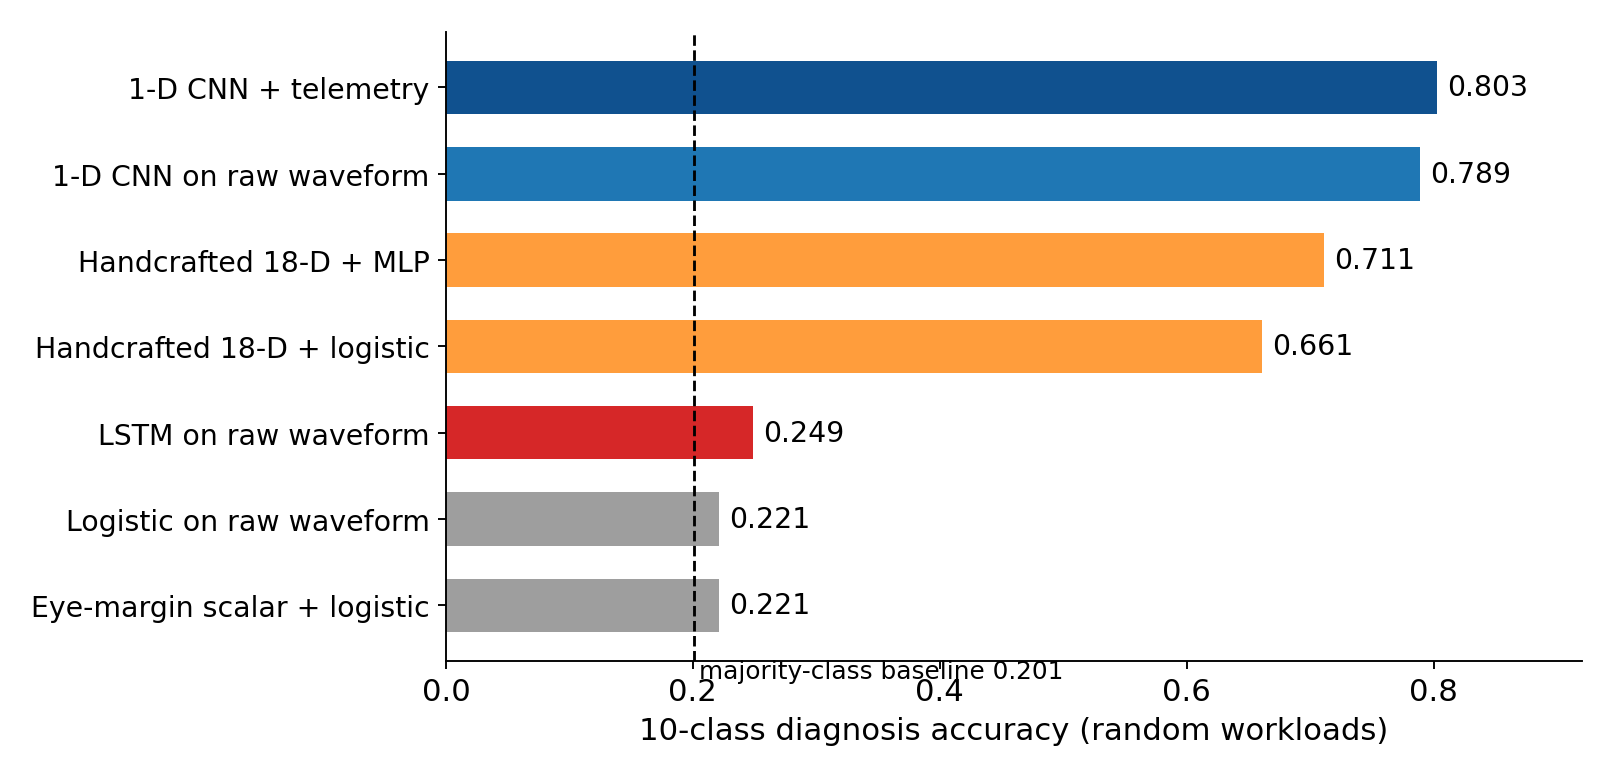
\includegraphics[width=0.95\textwidth]{pic/ladder.png}
    \end{figure}
    \begin{itemize}\small
        \item 随机码型使\hl{线性模型在原始波形上彻底失效}（0.221 $\approx$ 瞎猜）
        \item LSTM 同样崩溃（0.249）——起作用的是\hl{卷积的平移等变先验}，不是“深度”
    \end{itemize}
\end{frame}

\begin{frame}{残余混淆 = 物理机制简并}
    \begin{columns}
        \column{0.58\textwidth}
            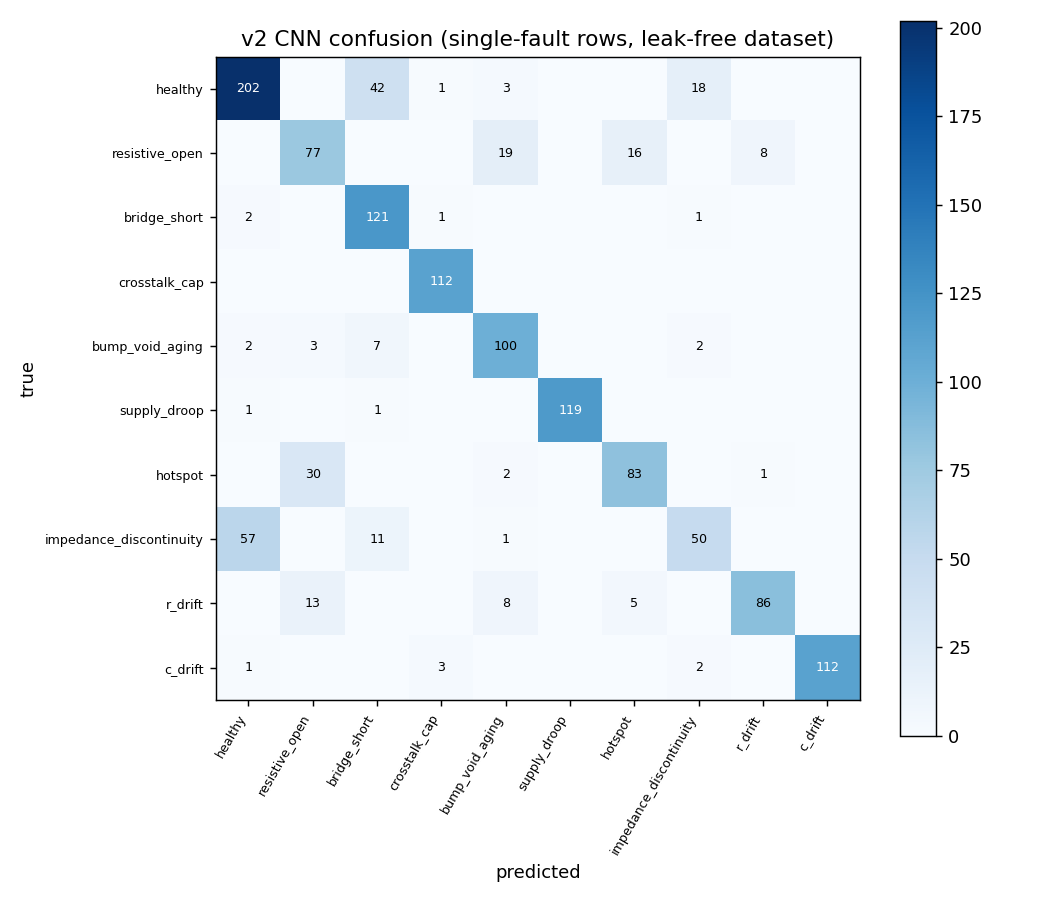
\includegraphics[width=\textwidth]{pic/confusion_v2.png}
        \column{0.40\textwidth}
            \small
            \begin{itemize}
                \item 弱阻抗台阶 $\leftrightarrow$ 健康：$z\to1$ 时电学上无差别
                \item hotspot $\to$ resistive\_open：同为局部串阻升高
                \item resistive\_open $\leftrightarrow$ bump\_void：取值区间\hl{有意重叠}（20--80 $\Omega$）
            \end{itemize}
            \vspace{0.5em}
            混淆不是模型缺陷，而是\hl{观测的物理上限}
    \end{columns}
\end{frame}

\begin{frame}{判别信息住在哪里：区域消融}
    \begin{figure}
        \centering
        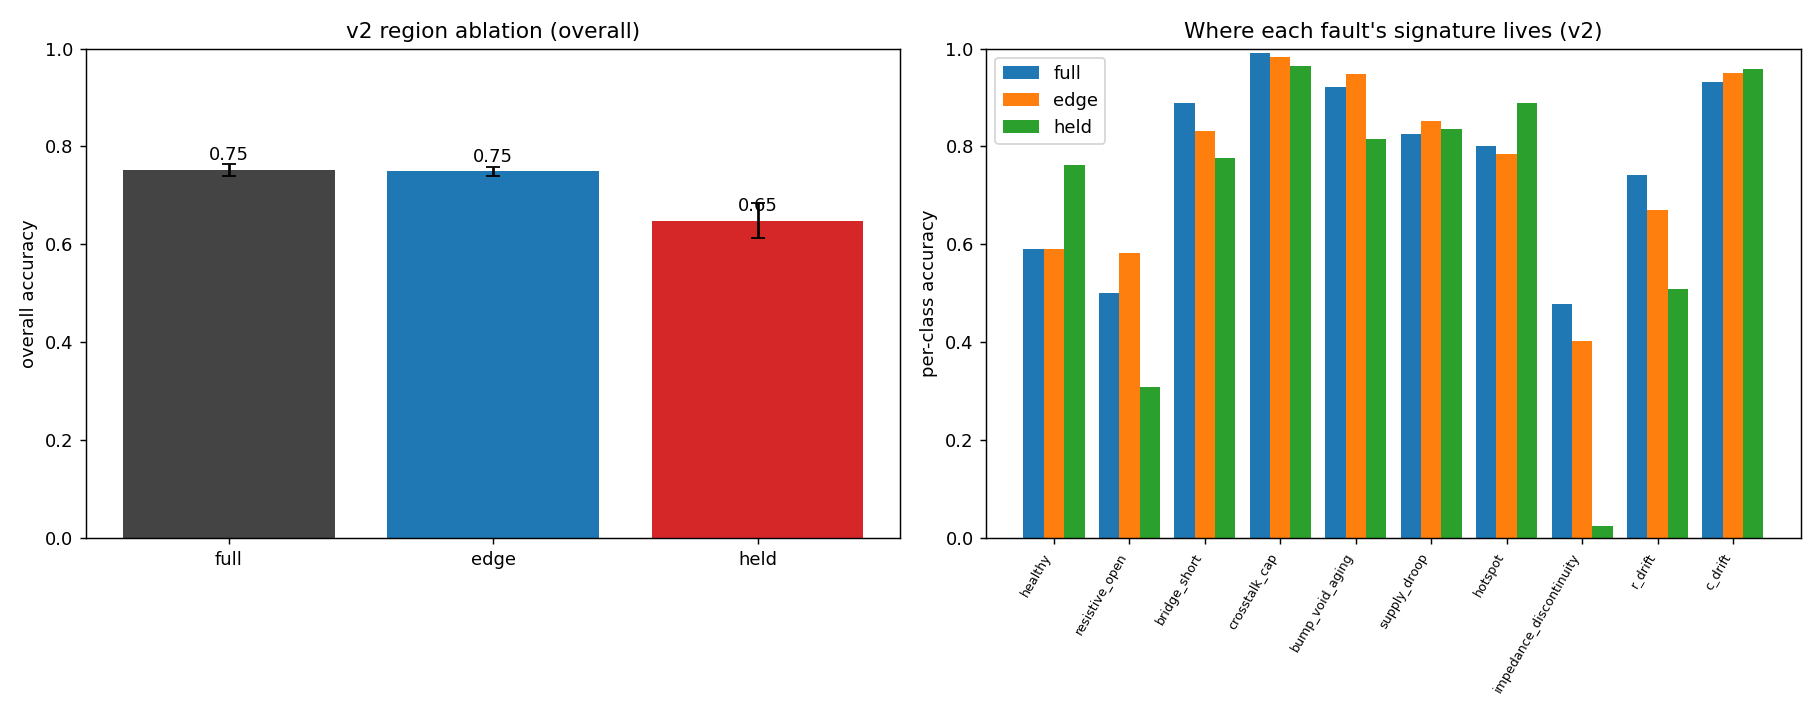
\includegraphics[width=0.99\textwidth]{pic/region_ablation_v2.png}
    \end{figure}
    \begin{itemize}\small
        \item 仅保留\hl{跳变沿}区 $\approx$ 全波形（0.749 vs 0.752）；仅平台区掉 10 个点
        \item 反射域故障（阻抗台阶）平台区坍缩到 \hl{0.03}——按沿对齐采样 $>$ 均匀降采样
    \end{itemize}
\end{frame}

\begin{frame}{混杂长什么样：运行时只有一个标量时}
    \begin{columns}
        \column{0.55\textwidth}
            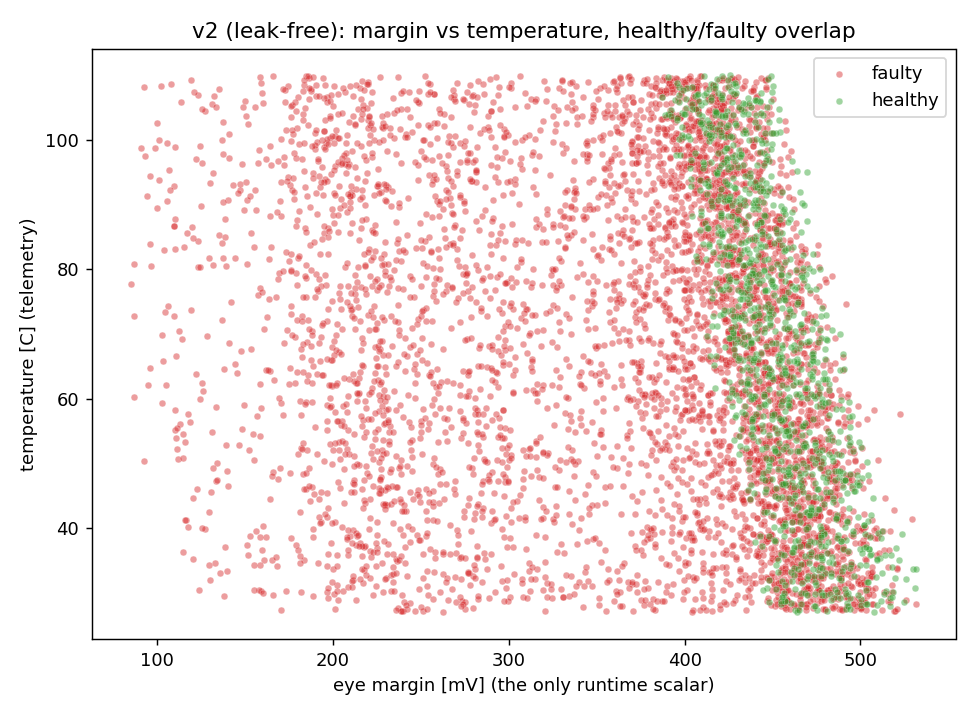
\includegraphics[width=\textwidth]{pic/lossy_confounder_v2.png}
        \column{0.43\textwidth}
            \small
            \begin{itemize}
                \item 横轴：运行时唯一可得的\hl{眼裕度标量}
                \item 健康（绿）随温度整体左移——$R_\text{on}(T)$ 闭眼
                \item 任何单一阈值：要么漏检，要么\hl{误报高温健康链路}
            \end{itemize}
            \vspace{0.4em}
            加入温度维度后，“裕度低但温度高”可被解释为\hl{良性}
    \end{columns}
\end{frame}

\begin{frame}{核心洞见：遥测的价值取决于观测的有损性}
    \begin{figure}
        \centering
        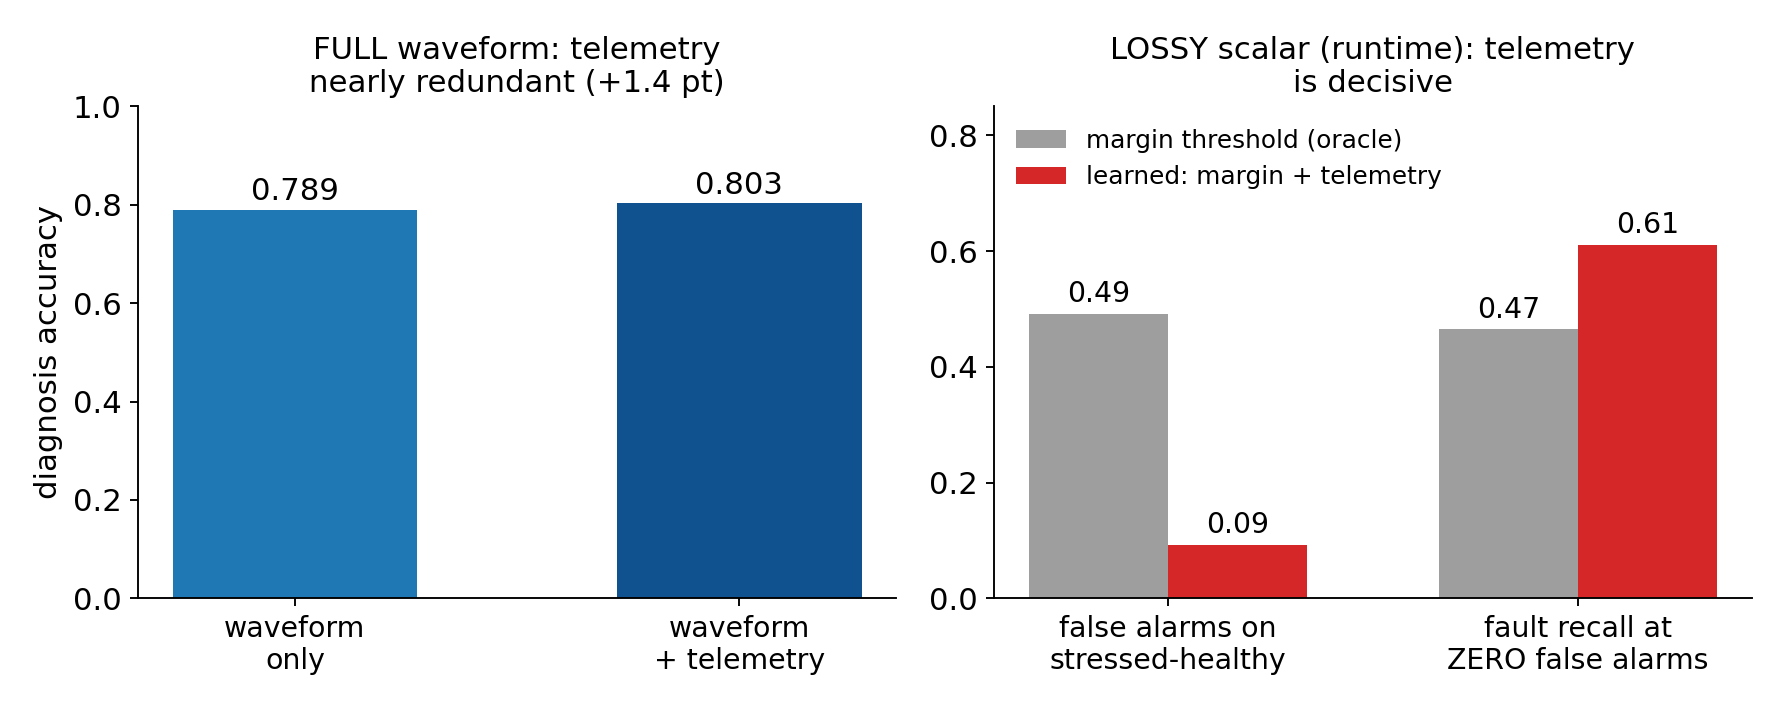
\includegraphics[width=0.97\textwidth]{pic/telemetry_value.png}
    \end{figure}
    \begin{center}
        \small 完整波形已隐含混杂变量 $\Rightarrow$ 遥测近乎冗余；\\
        观测越有损，\hl{多模态融合越是必需}——“多加遥测总更好”并不成立
    \end{center}
\end{frame}

\begin{frame}{其他结果：严重度、并发故障、码型泛化}
    \centering
    \begin{tabular}{@{}lll@{}}
        \toprule
        任务 & 指标 & 结果 \\
        \midrule
        r\_drift 严重度回归 & $R^2$ & \textbf{0.894} \\
        c\_drift 严重度回归 & $R^2$ & \textbf{0.908} \\
        多标签并发诊断 & macro-F1 & \textbf{0.72} \\
        未见过的 PRBS 码型 & 精确匹配 & 0.581（随机划分 0.542） \\
        \bottomrule
    \end{tabular}
    \vspace{0.8em}
    \begin{itemize}\small
        \item 在制造偏差 + 抖动 + 随机码型全部滋扰下，严重度仍可回归到 $R^2\approx0.9$\\
              $\Rightarrow$ 支撑“在 BER 恶化之前量化退化”的潜伏故障监测
        \item 跨随机码型训练\hl{本身}就带来码型不变性——无需显式 TX 条件输入
    \end{itemize}
\end{frame}

\begin{frame}{诚实的负结果：未知故障检测不可用}
    \begin{columns}
        \column{0.52\textwidth}
            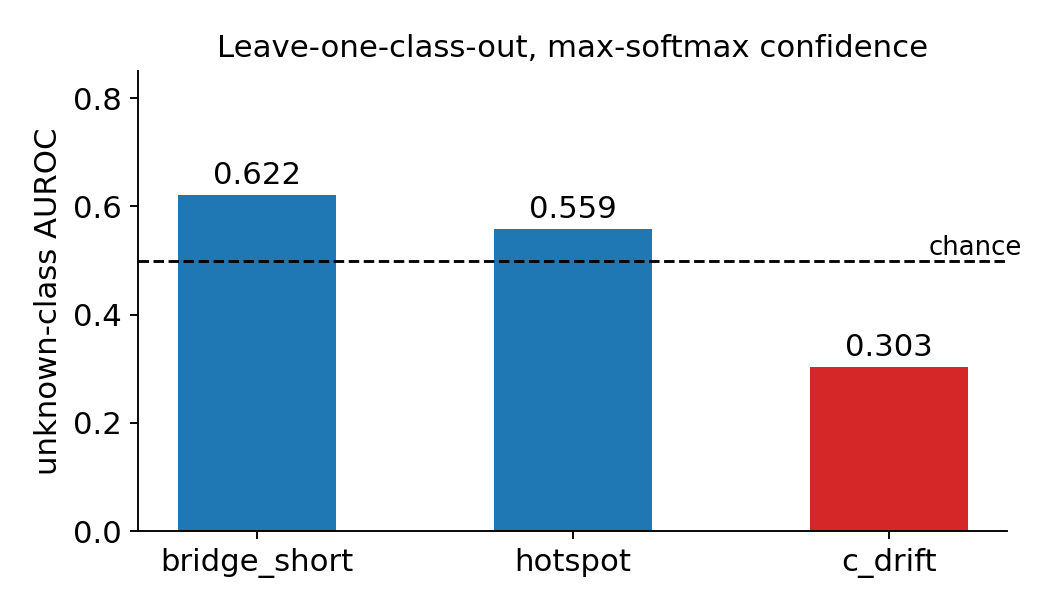
\includegraphics[width=\textwidth]{pic/openset.png}
        \column{0.46\textwidth}
            \small
            \begin{itemize}
                \item 留一类实验：训练时移除某故障类，用 max-softmax 置信度认“未知”
                \item c\_drift 的 AUROC 仅 \hl{0.303}：未知样本被\hl{自信地}吸收进相近已知类
                \item 在役部署前必须补充显式 OOD 检测（重构误差/密度估计）
            \end{itemize}
    \end{columns}
\end{frame}

% ============================================================
\section{结论与展望}

\begin{frame}{局限}
    \begin{itemize}
        \item 仿真数据，物理参数有文献依据但\hl{未经实测硅校准}
        \item 接收端为无源探测：不含 CTLE/DFE 均衡与 CDR——结论属于“焊盘原始波形”体制
        \item 运行时的真实观测是误码序列/裕度计数，比本文的标量更粗
        \item 多标签报警的健康误报偏高 $\Rightarrow$ 需二分类健康门把守
        \item 开集识别是公开的未解项
    \end{itemize}
\end{frame}

\begin{frame}{结论：三句话}
    \begin{enumerate}
        \item 随机工作负载下，\hl{从原始信号学习表征是必需}：线性模型 0.221 $\to$ CNN 0.789，且结构要匹配信号（LSTM 0.249）
        \item \hl{遥测的价值取决于观测的有损性}：完整波形下 +1.4 pt；有损标量下高应力误报 49\%$\to$9\%、零误报检出 46.5\%$\to$61.1\%
        \item 全部基于开源 ngspice + Python，6000 样本 20 分钟可复现——一个\hl{可证伪}的 D2D 在役诊断基准
    \end{enumerate}
    \vspace{0.8em}
    \begin{center}
        \small 代码与数据：\url{https://github.com/Yuanqi1231/VLSI-Testing}
    \end{center}
\end{frame}

\begin{frame}
    \begin{center}
        {\Huge\calligra Thanks!}
    \end{center}
\end{frame}

\end{document}
